% !TEX TS-program = XeLaTeX
% Commands for running this example:
% 	 xelatex Seamless_Blending
% 	 xelatex Seamless_Blending
% End of Commands
\documentclass[11pt,a4paper,twocolumn]{article}
% Mahmood Amintoosi
% محمود امین طوسی - دانشگاه علم و صنعت ایران - مقاله آماده شده برای کنفرانس کامپیوتر
% فایلهایی که در تهیه گزارشات این مقاله مورد استفاده قرار گرفته اند به قرار زیرند:
% Directory: D:\PhDCourses\SuperResolution\LK-SSIM-LM
%در این قسمت من برنامه های MATLAB ی که برای این مقاله نوشته ام را یادداشت می کنم که در مراجعات بعدی فراموش نکنم.

\usepackage{algorithm}
\usepackage{algorithmic}
\usepackage{pdfsync}
\usepackage{graphicx}
\usepackage{subfigure}
%\usepackage{backref}

\usepackage{pstricks}
\usepackage{animate}
\usepackage{pstricks-add}
\usepackage{multido}
\usepackage{color}
\usepackage{fancybox}
\usepackage{fancyvrb}
\usepackage{setspace}
\usepackage{amsmath}
\usepackage[colorlinks,citecolor=blue]{hyperref}
\usepackage[top=25mm, bottom=25mm, left=20mm, right=20mm]{geometry}

\setlength{\columnwidth}{82mm}
\setlength{\columnsep}{6mm}

\usepackage{bidipoem}

\usepackage{xepersian}
\settextfont[Scale=1]{XB Niloofar}%{B Nazanin}%
\setlatintextfont[Scale=.9]{Times New Roman}
%\setdigitfont{XB Zar}
\defpersianfont\iranic[Scale=.8]{XB Zar Italic}
%\defpersianfont\Keyhan[Scale=1]{XB Kayhan Sayeh}

\defpersianfont\TitleBold[Scale=1]{XB Niloofar Bold}
\defpersianfont\AbstractBold[Scale=.92]{XB Niloofar Bold}
\defpersianfont\nastaliq[Scale=1.2]{IranNastaliq}
%\usepackage{persianpoem}


\newcommand{\textblue}[1]{{\addfontfeature{Color=0000FF}#1}}
\numberwithin{table}{section}
\onehalfspacing

\newcommand\femph[1]{\lr{''}#1\lr{``}}

\renewcommand{\algorithmicrequire}{\textbf{ورودی:}}
\renewcommand{\algorithmicensure}{\textbf{خروجی:}}


\begin{document}

\title{\TitleBold{همرنگ‌سازی چند بانده+آمیختن مبتنی بر موجک در وضوحِ برتر}}

\author{محمود امین طوسی$^{\ddag,\dag}$، محمود فتحی$^\dag$ و ناصر مزینی$^\dag$\\
$^\dag$دانشگاه علم و صنعت ایران، دانشکده مهندسی کامپیوتر\\
$^\ddag$ دانشگاه حکیم سبزواری، گروه ریاضی\\  
\lr{\{mAmintoosi,mahFathy,Mozayani\}@iust.ac.ir}\\
{\shadowbox{\textblue{
 این مقاله کامل نیست و فقط به عنوان یک نمونه از مقالات آماده شده با زی‌پرشین آورده شده است}} }\\
}

\twocolumn[
\thispagestyle{empty}
%%%%%%%%% ABSTRACT
\begin{@twocolumnfalse}
\date{}
\pagestyle{empty}
\maketitle\thispagestyle{empty}
\begin{abstract}
\AbstractBold
{ آمیختن\LTRfootnote{ Fusion} عبارت است از ایجاد یک تصویر از ترکیب دو یا چند تصویر دیگر، به نحوی که اطلاعات مهم آنها محفوظ بماند. 
آمیختن تصاویر به نحوی که مرز تصاویر آشکار نباشد یکی از موضوعات مهم در مسائل وضوحِ برتر\LTRfootnote{ Super-Resolution} و تصاویر عریض\LTRfootnote{ Panorama} می‌باشد. در این مقاله شیوه‌ای ترکیبی بر اساس روشهای همرنگ‌سازی چند بانده، مبتنی بر هرم لاپلاسین و تبدیل موجک برای آمیختن بدون درز تصاویر ارائه شده است. شیوه‌ی پیشنهادی در حالتی خاص از مسئله‌ی وضوحِ برتر بکار گرفته شده است. هدف در مسئله‌ی موردنظر، افزایش وضوح یک ناحیه از تصویر ورودیِ با وضوح پایین با استفاده از یک تصویر آموزشیِ با وضوح بالاست.  نتایج پیاده‌سازی‌های انجام شده برتری شیوه‌ی پیشنهادی را در مقایسه با هر یک از دو روش همرنگ‌سازی چندبانده و تبدیل موجک نشان می‌دهد.}
 \end{abstract}
 \hspace{9mm}\textbf{کلمات کلیدی}: آمیختن، ثبت تصویر، موجک، وضوح برتر، هم‌رنگ‌سازی.\\

\end{@twocolumnfalse}]

\section{مقدمه}

به فرآیند ترکیب\LTRfootnote{ Combination} اطلاعات دو یا چند تصویر از یک صحنه، جهت حصول یک تصویر که دارای اطلاعات 
بیشتری بوده و برای درک بصری یا پردازش کامپیوتری مناسب‌تر است «آمیختن \LTRfootnote{ Fusion}» گفته می‌شود
\cite{Goshtasby07image}. معمولاً تصاویر مورد ترکیب با استفاده از حسگرهای مختلف اخذ شده و با هم آمیخته می‌شوند.
اما آنچه که در این مقاله مدنظر است ترکیب تصاویری با وضوح‌، رنگ و زاویه‌ی اخذ متفاوت از یک صحنه می‌باشد. 

آمیختن تصویر به سه سطح: پایین، میانه و بالا تقسیم‌بندی می‌شود که برخی به آنها به عنوان سطوح پیکسلی، ویژگی 
و نمادین\LTRfootnote{ Symbolic} اشاره می‌کنند. برخلاف  سطح اول (پایین)، کارهای کمی  در زمینه‌ی
دو سطح دیگر انجام شده است. متدهای مبتنی بر ویژگی معمولاً تصویر را به چند ناحیه قطعه‌بندی نموده و 
نواحی را با استفاده از خصوصیات مختلفشان ترکیب می‌کنند. این متدها معمولاً حساسیت کمتری به نویز دارند.
متدهای سطح بالا، توصیف کننده‌های تصویر -مانند گرافهای رابطه‌ای
%\LTRfootnote{ Relational graphs}
-را آمیخته می‌کنند
\cite{Goshtasby07image}.%,Wang07framework

یکی از مشهورترین آثار در حوزه‌ی ترکیب تصاویر را می‌توان تکنیک هرم لاپلاسیِن \lr{Burt}\cite{Burt83multiresolution} دانست که از روشهای سطح پیکسلی به‌شمار می‌رود. در این روش از سطوح مختلف تفکیک‌پذیری\LTRfootnote{ Resolution} برای آمیختن تصاویر در مسئله‌ی موزائیک تصاویر\LTRfootnote{ Photo mosaic} بهره گرفته شده است. 
یکی از زیر مسائل این تکنیکها و تصاویر عریض\LTRfootnote{ Panorama}، ترکیب دو تصویر به نحوی است که لبه‌های تصاویر در ناحیه‌ی هم‌پوشان مشخص نباشد.  حتی تفاوت سطح خاکستری در مرز ناحیه‌ی هم‌پوشان به خوبی قابل رؤیت می‌باشد. لذا نیازمند روشی برای ترکیب هستیم که انتقال از یک تصویر به تصویر دیگر به نرمی صورت پذیرفته، مرز دو تصویر دیده نشود و در عین حال اطلاعات تصاویر اصلی تا حد امکان محفوظ بماند. به چنین روش ترکیبی، ترکیب بدون درز\LTRfootnote{ Seamless} گفته می‌شود.

ساده‌ترین راه حذف درز را می‌توان روش میانگین‌گیری وزن‌دار پیکسلهای دو تصویر در ناحیه‌ی هم‌پوشان دانست. فرض کنید تصویر $A$ در سمت چپ و تصویر $B$ در سمت راست بوده، $A(i)$ پیکسل $i$ام ناحیه‌ی هم‌پوشان در تصویر سمت چپ، $B(i)$ پیکسل متناظر از تصویر سمت راست و $\hat{i}$ مختصات پیکسل روی مرز باشد. همچنین به فرض $H_l(i)$ تابع وزن‌دهی باشد که نزولی یکنوا از چپ به راست بوده و $H_r(i) = 1-H_l(i)$ باشد. تصویر ترکیبی $S$ به صورت زیر بدست خواهد آمد:
\begin{equation}
S(i) = H_l(i-\hat{i})A(i) + H_r(i-\hat{i})B(i)
\end{equation}

\floatname{algorithm}{\rl{الگوریتم}}
\begin{algorithm}[t]
\caption{الگوریتم آمیختن تصاویر $A$ و $B$  با تکنیک هرم لاپلاسین \cite{Burt83multiresolution}.} \label{alg1}
\begin{algorithmic}[1]
\REQUIRE تصاویر $A$ و $B$.\\
\ENSURE تصویر $S$ حاصل از آمیختن نیمه‌ی سمت چپ $A$ و نیمه‌ی سمت راست $B$
  \STATE هرمهای لاپلاسین $LA,LB$ از تصاویر $A,B$ ساخته می‌شوند.
  \STATE هرم لاپلاسین سومی به نام $LS$ با کپی کردن نیمه‌های سمت چپ $LA$ و سمت راست $LB$ ساخته می‌شود. عناصر ستون وسط $LS$ با میانگین‌گیری از عناصر نظیر آنها در $LA,LB$ بدست می‌آیند. 
  \STATE تصویر نهایی $S$ با گسترش هر سطح هرم $LS$ و جمع آن با سطح بعدی حاصل خواهد شد.   
\end{algorithmic}
\end{algorithm}

انتخاب مناسب تابع $H$ باعث خواهد شد که انتقالی نرم از یک تصویر به دیگری داشته باشیم. ولی ناپیدا بودن درز را تضمین نمی‌کند. فرض کنید $T$ پهنای ناحیه‌ی هم‌پوشان باشد که در آن $H_l$ از یک به صفر تغییر می‌نماید. اگر $T$ در مقایسه با اندازه‌ی ویژگیهای تصاویر کوچک باشد، درز قابل رؤیت خواهد بود. از طرف دیگر اگر $T$ بزرگ باشد، دو تصویر شبیه به وضعیتی که دو عکس روی یک فیلم گرفته شده باشند، با هم ادغام می‌شوند. 
این مجموعه تصاویر بدست آمده با  فیلتر پایین‌گذر، هرم گوسین\LTRfootnote{ Gaussian pyramid} نامیده می‌شود. برای ساخت تصاویر فیلتر شده با یک فیلتر میان‌گذر، کافیست که هر سطح از هرم فوق‌الذکر از سطح پایینی خود کم شود. البته چون ابعاد دو سطح با هم متفاوت است، تصویر هر سطح قبل از تفریق به اندازه‌ی تصویر سطح بعدی گسترش داده می‌شود. تصاویر در این ساختار هرمی جدید را با $L_0,L_1,\dots,L_N$ نمایش داده و هرم لاپلاسین\LTRfootnote{ Laplacian pyramid} نامیده می‌شود. 

فرض کنید هدف آمیختن نیمه‌ی سمت چپ تصویر $A$ و نیمه‌ی سمت راست تصویر $B$ باشد. همچنین به فرض هر دو تصویر مربعی بوده و هر ضلع $2^N$ پیکسل داشته باشد. تصویر آمیخته نهایی با استفاده از الگوریتم \ref{alg1} ساخته می‌شود.

یک دسته‌ی مشهور دیگر از تکنیک‌های آمیختن، روشهای مبتنی بر تبدیل موجک است
 \cite{Hill02image,Nikolov01wavelets,Piella03thesis}.
آمیختن با تبدیل موجک را می‌توان با $\omega$، تبدیل موجکِ دو تصویر و قانونِ آمیختن $\phi$ بیان نمود.
تصویر آمیخته‌ ی $I(\mathbf{x})$، با استفاده از تبدیل موجک $\omega$، معکوس آن $\omega^{-1}$ و قانون $\phi$  به صورت زیر حاصل می‌شود:
\begin{equation}\label{eq:DWT_Fusion}
I(\mathbf{x})=\omega^{-1}\Big( \phi \big(
\omega(I_1(\mathbf{x})),\omega(I_2(\mathbf{x}))\big)\Big) \end{equation}
شکل \ref{fig:DWT_Fusion} نمایش شماتیک این روش را نشان می‌دهد. از آنجا که ضرائب موجک با قدرمطلق بزرگ، حاوی اطلاعات نمایان و مهم تصویر همچون لبه‌ها و خطوط هستند، یک قانون آمیختن خوب می‌تواند انتخاب بیشینه‌ی ضرائب متناظر دو تصویر باشد. 

اخیراً نویسندگان در \cite{Amintoosi08reconstruction,Amintoosi09regional} شیوه‌ای مشتمل بر استفاده از تصاویر آموزشی با وضوح بالا را برای افزایش وضوح تصویر ورودی ارائه نموده‌اند؛ لیکن در آثار مذکور مرحله‌ی همرنگ نمودن\LTRfootnote{ Blending} تصاویر مورد ترکیب، بدون درز نبوده است. در این مقاله با استفاده از ترکیب روش همرنگ‌سازی چند بانده
\LTRfootnote{ Multi-band Blending}
(هرم لاپلاسین) و تبدیل موجک این نقیصه برطرف شده است.

%------------------------- DWT_Fusion
\begin{figure}[t]
\centering 
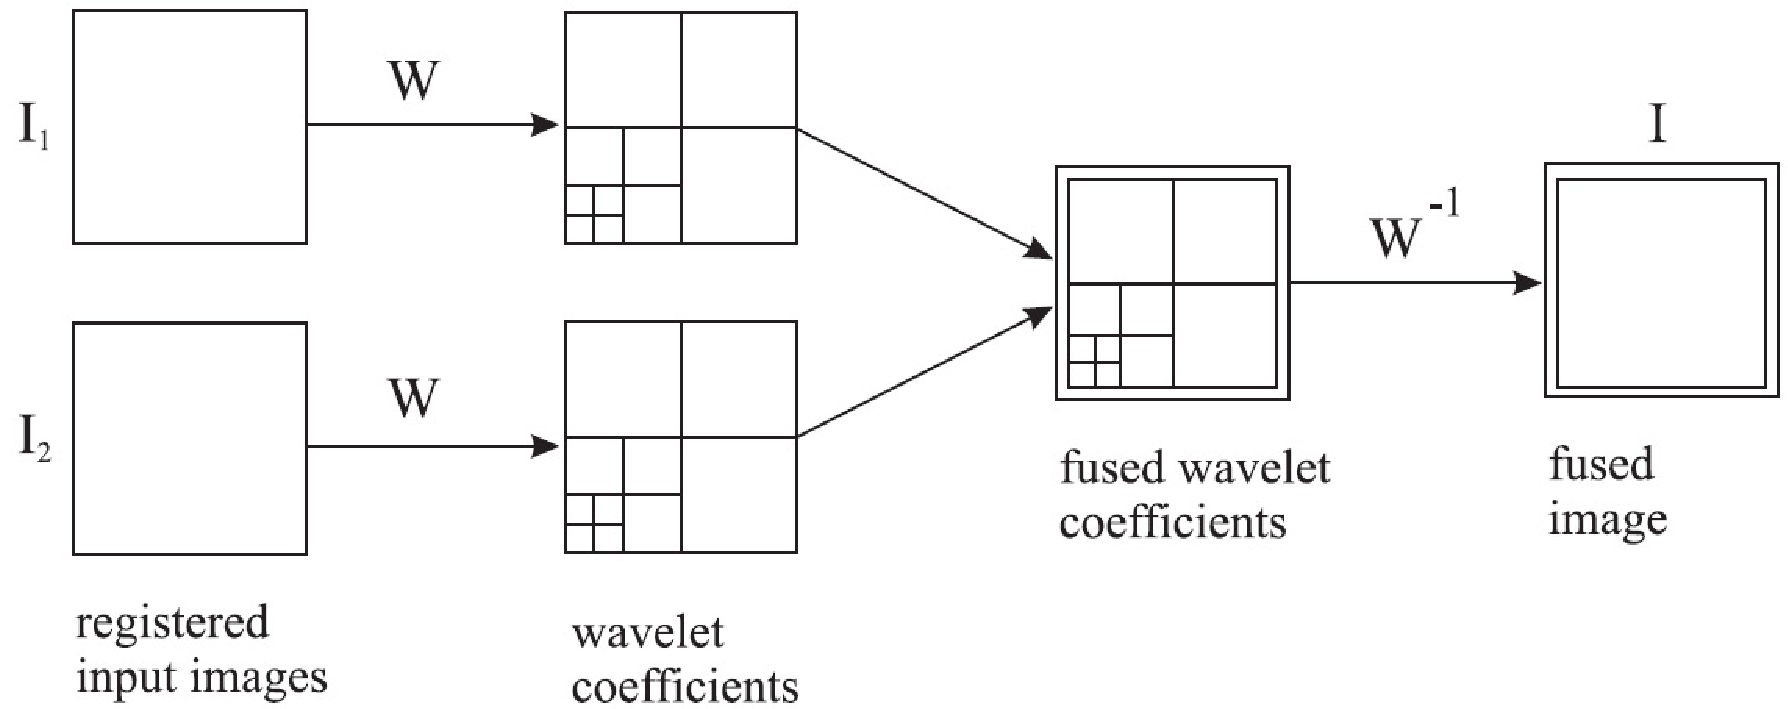
\includegraphics[width=80mm]{Images/DWT_Fusion.pdf}
\caption{نمایش شماتیک آمیختن با تبدیل موجک \cite{Nikolov01wavelets}.}\label{fig:DWT_Fusion}
\end{figure}

  
در بخش \ref{Sec:TheProposedMethod} شیوه‌ی پیشنهادی، در بخش \ref{Sec:ExperimentalResults} نتایج پیاده‌سازی‌ها و در انتها جمع‌بندی آورده شده است.

%%%%%%%%%%%%%%%%%%%%%%%%%%%%%%% \section{شیوه‌ی پیشنهادی و نتایج}
\section{شیوه‌ی پیشنهادی}\label{Sec:TheProposedMethod}

 در شیوه‌ی پیشنهادی برای وضوح برتر توسط نگارندگان در \cite{Amintoosi08reconstruction}، هر یک از تصاویر باوضوح بالا، به عنوان تصویر آموزشی، متناظر با قسمتی از تصویرِ باوضوح پایین هستند.  تصاویر آموزشی می‌توانند تفاوتهایی با تصویر اصلی از نقطه نظر شدت روشنائی یا زاویه‌ی اخذ داشته باشند. 
% این تفاوتها می‌تواند ناشی از برداشت عکسها در زمانهای متفاوت و یا با دوربینهای متفاوت و از زوایای مختلف باشد.
 در این شیوه ابتدا تصویر با وضوح پایین به اندازه‌ی مطلوب بزرگ شده و سپس  تبدیل مناسبی برای نگاشت هر یک از تصاویر آموزشی بر روی تصویر مورد نظر با استفاده از  نقاط کلیدی \lr{SIFT}\LTRfootnote{ Scale Invariant Feature Transform (SIFT)} و الگوریتم \lr{RANSAC}\LTRfootnote{ RANdom SAmple Consensus (RANSAC)} در قالب ماتریس هوموگرافی
\LTRfootnote{ Homography matrix}
 پیدا می‌شود. 
 
%------------- تصاویر بیستون
\begin{figure}[tp]
\centering \subfigure[{تصویر ورودی}]{\label{fig:Katibeh:LR}
\includegraphics*[width = .24\columnwidth]{Images/Kamandar_LR_Nearest.jpg}}%\vspace{2mm}
\subfigure[{تصویر آموزشی}]{\label{fig:Katibeh:HR}
\includegraphics*[width = .24\columnwidth]{Images/Neyzeh_dar.jpg}}%\hspace{2mm}
\subfigure[{نتیجه نهایی }]{\label{fig:Katibeh:Final}
\includegraphics*[width = .48\columnwidth]{Images/Kamandar_blendXFus_FA.jpg}}
 \caption{مثال اول: تصاویری از نقش‌برجسته‌ی بیستون. نتیجه نهایی افزایش وضوح تصویر با وضوح پایین ورودی(آ) با استفاده از تصویر با وضوح بالای آموزشیِ(ب) و با روش پیشنهادی در این مقاله در شکل (ج) نشان داده شده است. برای مقایسه‌ی بهتر تصویر ورودی و تصویر نهایی به شکل \ref{fig:KatibehResults} رجوع نمایید.}
\label{fig:Katibeh}
\end{figure}

\section{نتایج پیاده‌سازی}\label{Sec:ExperimentalResults}

برای نمایش کارائی شیوه‌ی پیشنهادی دو مثال ذکر شده است. در هر مثال یک تصویر ورودی با وضوح پایین و یک تصویر با وضوح بالا داریم که نمایانگر قسمتی از تصویر ورودی است. دو تصویر از منظر رنگ‌بندی، وضوح و زاویه‌ی اخذ تفاوتهایی با یکدیگر دارند. هدف ما بالابردن وضوح قسمت متناظر با تصویر با وضوح بالا  در تصویر ورودی است. ضریب بزرگ‌نمایی، 2 در نظر گرفته شده است. 

تصاویر مورد استفاده در مثال اول در شکل‌های \ref{fig:Katibeh:LR} و \ref{fig:Katibeh:HR} نشان داده شده‌اند. این تصاویر از یکی از سی‌دی‌های مربوط به نقش برجسته‌ی داریوش در بیستون اخذ شده‌اند. همانگونه که در شکل \ref{fig:Katibeh} مشاهده می‌شود دو تصویر از نظر وضوح، شدت روشنایی و رنگ‌بندی با یکدیگر متفاوت هستند.  شکل \ref{fig:Katibeh:Final} نتیجه‌ی نهائی افزایش وضوح تصویر \ref{fig:Katibeh:LR} با استفاده از تصویر آموزشی \ref{fig:Katibeh:HR} را نشان می‌دهد. 

\begin{figure}[t]
\centering 
\subfigure[\rl{روش بزرگنمائي} \lr{Bicubic}]{ \label{fig:KatibehResults:Bicubic}
\lr{\includegraphics[width=35mm]{Images/Kamandar_LR_Cropped.jpg}}}
\hspace{2mm}
\subfigure[\rl{روش  هرم لاپلاسین \cite{Burt83multiresolution}}]{\label{fig:KatibehResults:LaplacianPyramid}
\lr{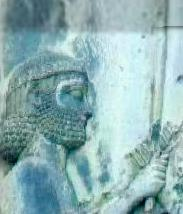
\includegraphics[width=35mm]{Images/Kamandar_blend_FA_cropped.jpg}}}
\hspace{2mm}
\subfigure[\rl{روش   مبتنی بر تبدیل موجک استفاده شده در \cite{Amintoosi08reconstruction} } ]{ \label{fig:KatibehResults:DWT}
\lr{\includegraphics[width=35mm]{Images/Kamandar_Fustruction_Cropped.jpg}}}
\hspace{2mm}
\subfigure[\rl{روش  پيشنهادي در اين مقاله}]{\label{fig:KatibehResults:DWT_LaplacianPyramid}
\lr{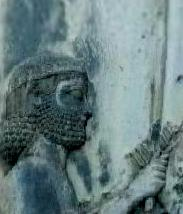
\includegraphics[width=35mm]{Images/Kamandar_blendXFus_FA_cropped.jpg}}}
\caption{\rl{بزرگ شده‌ي قسمتي از نتيجه‌ي اجراي شيوه‌هاي مختلف براي افزايش وضوح شکل \ref{fig:Katibeh:LR} با استفاده از آمیختن تصویر آموزشیِ \ref{fig:Katibeh:HR} .}}
\label{fig:KatibehResults} %% label for entire figure
\end{figure}

برای مقایسه‌ چند شیوه‌ی دیگر پیاده‌سازی شده‌اند و یک ناحیه از هریک در شکل \ref{fig:KatibehResults} برای مقایسه بزرگ شده است. مقایسه‌ی تصاویر شکل اخیر کیفیت برتر شیوه‌ی پیشنهادی را برای این مثال به خوبی نشان می‌دهد.  ناپدید شدن درز در نواحی مرزی در شیوه‌ی پیشنهادی مشخص است. همانگونه که دیده می‌شود در آمیختن با تکنیک هرم لاپلاسین (شکل \ref{fig:KatibehResults:LaplacianPyramid}) تغییر رنگ کاملاً واضح است. در روش مبتنی بر موجک استفاده شده در \cite{Amintoosi08reconstruction} (شکل \ref{fig:KatibehResults:DWT}) مرز تصویر ترکیب شده قابل رؤیت است. 
%در شیوه‌ی پیشنهادی (شکل \ref{fig:KatibehResults:DWT_LaplacianPyramid}

شکل‌ \ref{fig:BooAliSina} مثال دوم را نشان می‌دهد که تصاویری با وضوح پایین و با وضوح بالا از آرامگاه ابوعلی سینا در همدان هستند. تصاویر با دوربین \lr{Panasonic NV-GS75} توسط نگارنده اخذ شده‌اند. تصویر با وضوح بالاتر (شکل \ref{fig:BooAliSina:HR}) از سنگ‌نوشته‌ی حاوی قطعه شعری از ابوعلی سینا با زووم کردن اُپتیکال گرفته شده است. متن این قطعه شعر در زیر آمده است:
%\begin{RTL}
{\nastaliq
\begin{traditionalpoem}
از قعر گل سیاه تا اوج زحل & 
کردم همه مشکلات عالم را حلّ\\
برون جستم ز قید هر مکر و حیل&
هر بند گشوده شد مگر بند اجل\\
\end{traditionalpoem}
}
. این قطعه شعر در تصویر \ref{fig:BooAliSina:LR} حتی با بزرگ نمودن آن (تصویر \ref{fig:BooAliSinaResults:Bicubic}) خوانا نیست. از آنجا که میزان نوردهی به صورت خودکار توسط دوربین مشخص می‌شود، تغییر شدت روشنایی و رنگ را بین دو تصویر شاهد هستیم. نتیجه‌ی نهایی ترکیب تصویر \ref{fig:BooAliSina:HR} با بزرگ شده‌ی \ref{fig:BooAliSina:LR}  در شکل \ref{fig:BooAliSina:Final} آمده است. مقایسه‌ی بهتر روشهای مختلف برای این مثال در شکل \ref{fig:BooAliSinaResults} دیده می‌شود.

%-------------------- بوعلی سینا
\begin{figure}[t]
\centering \subfigure[{تصویر ورودی}]{\label{fig:BooAliSina:LR}
\includegraphics*[width = .25\columnwidth]{Images/BooAliSina_LR_Nearest.jpg}}%\vspace{2mm}
\subfigure[{تصویرآموزشی}]{\label{fig:BooAliSina:HR}
\includegraphics*[width = .25\columnwidth]{Images/IMGA0142.JPG}}%\hspace{2mm}
\subfigure[{نتیجه نهایی }]{\label{fig:BooAliSina:Final}
\includegraphics*[width = .5\columnwidth]{Images/BooAliSina_blendXFus_FA.jpg}}
 \caption{مثال دوم: تصاویری از آرامگاه ابوعلی‌سینا. نتیجه نهایی افزایش وضوح تصویر با وضوح پایینِ ورودی(آ) با استفاده از تصویر با وضوح بالای آموزشیِ(ب) و با روش پیشنهادی در این مقاله در شکل (ج) نشان داده شده است. برای مقایسه‌ی بهتر تصویر ورودی و تصویر نهایی به شکل \ref{fig:BooAliSinaResults} رجوع نمایید.}
\label{fig:BooAliSina}
\end{figure}

\section{جمع‌بندی}\label{Sec:Conclusion}
% از جمله روشهای آمیختن می‌توان
% به روش میانگین‌گیری مقادیر پیکسلها، روشهای مبتنی بر آنالیز مؤلفه‌ی اصلی %\LTRfootnote{ Principal component analysis}
% و تبدیل موجک %\LTRfootnote{ Wavelet transform}
% اشاره نمود\cite{Goshtasby07image,Hill02image}.
 در ترکیب تصاویر با هم‌رنگ‌سازی چندبانده لبه‌ها محو می‌شوند، لیکن  تفاوت  تغییرات رنگیِ تصاویر نسبت به هم مشهود است؛ از طرفی با استفاده از تبدیل موجک، می‌توان رنگ را از یکی و اطلاعات با فرکانس بالا را از دیگری گرفت و مشکل اختلاف رنگ را نداریم ولی لبه‌ها کاملاً محو نمی‌شوند. ترکیب مناسب این دو الگوریتم در این مقاله به صورت ابتدا انجام ترکیب با شیوه‌ی مبتنی بر تبدیل موجک، ساخت یک ماسک مناسب و سپس استفاده از روش هم‌رنگ‌سازی چند بانده بر روی نتیجه‌ی مرحله‌ی اول صورت پذیرفته است. نتایج پیاده‌سازی‌های انجام شده برتری شیوه‌ی پیشنهادی را در مقایسه با هر دو روش مذکور، در حوزه‌ی وضوح برتر  نشان داده است.
 
\subsection*{سپاس‌گزاری}
مؤلفین وظیفه‌ی خود می‌دانند که از آقایان وفا خلیقی، دکتر مهدی امیدعلی و دکتر مصطفی واحدی
\LTRfootnote{\url{http://www.parsilatex.com}}
بابت زحمات و راهنمایی‌های ارزنده‌ی آنها در زمینه‌ی \lr{\XePersian} (بسته‌ی فارسی برای \lr{\LaTeX})  تشکر به عمل آورند. 

\begin{figure}[t]
\centering 
\subfigure[\rl{روش بزرگنمائي} \lr{Bicubic}]{ \label{fig:BooAliSinaResults:Bicubic}
\lr{\includegraphics[width=35mm]{Images/BooAliSina_LR_Cropped.jpg}}}
\hspace{2mm}
\subfigure[\rl{روش  هرم لاپلاسین \cite{Burt83multiresolution}}]{\label{fig:BooAliSinaResults:LaplacianPyramid}
\lr{\includegraphics[width=35mm]{Images/BooAliSina_blend_FA_Cropped.jpg}}}
\hspace{2mm}
\subfigure[\rl{روش  مبتنی بر تبدیل موجک استفاده شده در \cite{Amintoosi08reconstruction} } ]{ \label{fig:BooAliSinaResults:DWT}
\lr{\includegraphics[width=35mm]{Images/BooAliSina_Fustruction_Cropped.jpg}}}
\hspace{2mm}
\subfigure[\rl{روش  پيشنهادي در اين مقاله}]{\label{fig:BooAliSinaResults:DWT_LaplacianPyramid}
\lr{\includegraphics[width=35mm]{Images/BooAliSina_blendXFus_FA_Cropped.jpg}}}
\caption{بزرگ شده‌ي قسمتي از نتيجه‌ي اجراي شيوه‌هاي مختلف براي افزايش وضوح شکل \ref{fig:BooAliSina:LR} با استفاده از آمیختن تصویر آموزشیِ \ref{fig:BooAliSina:HR}}
\label{fig:BooAliSinaResults} %% label for entire figure
\end{figure}


\singlespacing
{\small
%\renewcommand{\refname}{\rl{{مراجع}\hfill}}

\setLTRbibitems
\begin{thebibliography}{9}
\resetlatinfont

\bibitem{Amintoosi08reconstruction}
M.~Amintoosi, M.~Fathy, and N.~Mozayani, ``Reconstruction+synthesis: A hybrid
  method for multi-frame super-resolution,'' in \emph{(MVIP08) 2008 Iranian
  Conference on Machine Vision and Image Processing}, University of Tabriz,
  Tabriz, Iran, pp. 179--184, Nov. 4-7 2008.

\bibitem{Amintoosi09regional}
------, ``Regional varying image super-resolution,'' in \emph{The 2009 IEEE
  International Joint Conference on Computational Sciences and Optimization
  (CSO 2009)}, Sanya, Hainan, China,Vol 1, pp. 913--917,  April 24-26 2009.

\bibitem{Burt83multiresolution}
P.~J. Burt and E.~H. Adelson, ``A multiresolution spline with application to
  image mosaics,'' \emph{ACM Trans. Graph.}, Vol.~2, No.~4, pp. 217--236, 1983.

\bibitem{Goshtasby07image}
A.~A. Goshtasby and S.~Nikolov, ``Image fusion: Advances in the state of the
  art,'' \emph{Inf. Fusion}, Vol.~8, No.~2, pp. 114--118, 2007.

\bibitem{Hill02image}
P.~Hill, N.~Canagarajah, and D.~Bull, ``Image fusion using complex wavelets,''
  in \emph{BMVC2002}, pp. 487--496, 2002.

%\bibitem{Wang07framework}
%Z.~hua Wang, Z.~Qin, and Y.~Liu, ``A framework of region-based dynamic image
%  fusion,'' \emph{Journal of Zhejiang University SCIENCE A}, Vol.~8, No.~1, pp.
%  56--62, 2007.

\bibitem{Nikolov01wavelets}
S.~Nikolov, P.~Hill, D.~Bull, and C.~Canagarajah, ``Wavelets for image
  fusion,'' in \emph{Wavelets in Signal and Image Analysis}.\hskip 1em plus
  0.5em minus 0.4em\relax Kluwer Academic Publishers, The Netherlands,
  ch. Wavelets for image fusion, pp. 213--244, 2001.

\bibitem{Piella03thesis}
G.~Piella, ``Adaptive wavelets and their applications to image fusion and
  compression,'' Ph.D. dissertation, Centre for Mathematics and Computer
  Science, University of Amsterdam, 2003.

\end{thebibliography}
}


\end{document}

